\documentclass{beamer}
\usetheme{Berlin}
\title{Nim}
\subtitle{Workshop: Programming Languages}
\author{Niklas Peter}
\institute{Universität Siegen}
\date{5. Februar 2024}
    
\usepackage{graphicx}
\begin{document}


\begin{frame}
\titlepage
\end{frame}


\begin{frame}
\frametitle{Inhalt}
\tableofcontents
\end{frame}


\begin{frame}
\frametitle{Allgemeines}
\section{Allgemeines}
\begin{itemize}
	\item Andreas Rumpf startete 2005 die Entwicklung
	\item Veröffentlichung in 2008 unter MIT Lizenz
	\item Version 1.0 kam am 23.09.2019 raus
	\item Soll effizient, ausdrucksvoll und elegant sein
	\item Generiert native ausführbare Programme ohne Abhängigkeiten
	\item Unterstützt BSD, Linux, macOS und Windows
\end{itemize}
\end{frame}


\begin{frame}
\frametitle{Design}
\section{Design}
\begin{itemize}
	\item Syntax inspiriert von Python
	\begin{itemize}
		\item Kennzeichnung von Codeblöcken durch Einrückung statt Klammern
		\item Schlüsselwörter (and, not, elif, ...)
		\item Kein Semikolon nach Statements
	\end{itemize}
	\item Style-Insensitive für Mischung verschiedener Stile:
	
	\emph{ein\_beispiel} und \emph{einBeispiel} sind gleich (nur erster Buchstabe muss übereinstimmen)
	\item Statische Typisierung aber mit einfacher Typumwandlung
	\item Uniform Function Call Syntax (UFCS)
	\begin{itemize}
		\item Funktionsaufruf durch Methoden-Syntax
		\item Receiver wird erster Parameter
		\item \emph{x = multiply(y, z)} entspricht \emph{x = y.multiply(z)}
	\end{itemize}
\end{itemize}
\end{frame}


\begin{frame}
\begin{itemize}
	\item Programmierungsparadigmen
	\begin{itemize}
		\item Funktionale Programmierung
		\item Objektorientierte Programmierung
		\begin{itemize}
			\item In erster Linie imperative und funktionale Sprache
			\item Grundlegende Elemente wie z.B. Polymorphie und Vererbung
		\end{itemize}
		\item Metaprogrammierung
		\begin{itemize}
			\item Templates
			\item Macros
			\item Generics
		\end{itemize}
		\item Foreign Function Interface (FFI)
		\begin{itemize}
			\item Zugriff auf in anderen Sprachen geschriebene Bibliotheken
		\end{itemize}
		\item Parallelisierung und Nebenläufigkeit
		\begin{itemize}
			\item Funktionen müssen gekennzeichnet werden
			\item Kompilierer benötigt \emph{-threads:on} Option
			\item Gewisse Regeln wie Einschränkung der Speicherzugriffe
		\end{itemize}
	\end{itemize}
\end{itemize}
\end{frame}


\begin{frame}
\begin{figure}[htp]
\centering
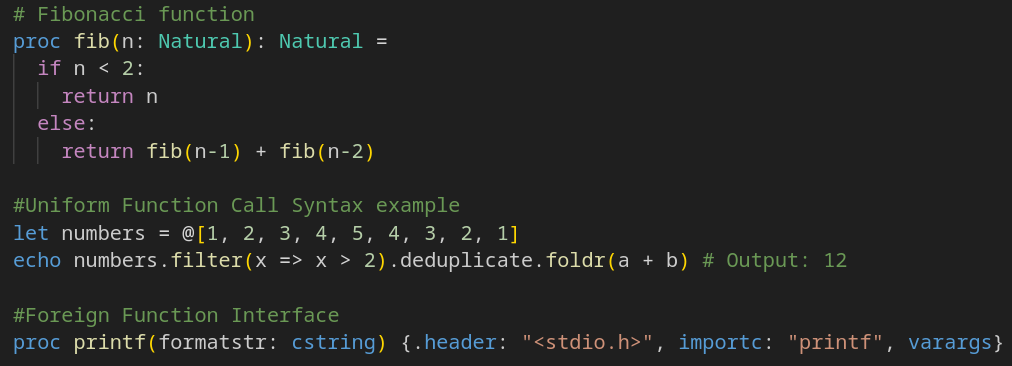
\includegraphics[scale=0.3]{Code Example.png}
\caption{Code Beispiel}
\label{}
\end{figure}
\end{frame}


\begin{frame}
\frametitle{Infrastruktur}
\section{Infrastruktur}
\begin{itemize}
	\item Kompilierer
	\begin{itemize}
		\item Vollständig in Nim geschrieben
		\item Gibt optimierten C Code aus. Kompilierung zu C++, Objective-C und JavaScript ebenfalls möglich
		\item Objektcode durch externen Kompilierer wie GCC
		\item Verschiedene Garbage Collectors verfügbar
		\begin{itemize}
			\item Standardmäßig Garbage Collector mit Referenzzählung
			\item Deaktivierung des Garbage Collectors möglich
		\end{itemize}
	\end{itemize}
\end{itemize}
\end{frame}


\begin{frame}
\begin{itemize}
	\item Entwicklungswerkzeuge (Auswahl)
	\begin{itemize}
		\item Nim's Paketmanager Nimble
		\item Nimsuggest zur Integration in IDEs
		\item Hot code reloading zum Neuladen des Codes zur Laufzeit
	\end{itemize}
	\item Bibliotheken
	\begin{itemize}
		\item Pure und Impure Bibliotheken
		\item Standardbibliothek mit grundlegenden Funktionen vollständig in Nim geschrieben
		\item Einbindung von Bibliotheken in C, C++, Objective-C und JavaScript möglich
		\item Kein zentrales Repository; jeder kann eigenes hosten
	\end{itemize}
\end{itemize}
\end{frame}


\begin{frame}
\frametitle{Anwendungsfälle}
\section{Anwendungsfälle}
Viele Einsatzmöglichkeiten durch Kompilierung nach C, C++ und JavaScript:
\begin{itemize}
	\item Shell Scripting
	\item Front- und Backend für Webdienste
	\item Machine Learning
	\item Eingebettete Systeme
\end{itemize}

Prominentes Beispiel ist \textbf{nitter}, ein Frontend für X (Twitter)
\end{frame}


\begin{frame}
\frametitle{Stärken und Schwächen}
\section{Stärken und Schwächen}
\begin{itemize}
	\item Einfache und flexible Syntax
	\item Moderne Konzepte
	\item Viele Anwendungsbereiche
	\item Nicht für alles eine native Bibliothek vorhanden, dafür aber Import von Bibliotheken in anderen Sprachen möglich
	\item Gute Dokumentation
	\begin{itemize}
		\item Ausführliche Dokumentation der Standardbibliothek
		\item Zahlreiche Tutorials für Neulinge
		\item Aktive Community in Foren und Chats
	\end{itemize}
\end{itemize}
\end{frame}


\begin{frame}
\frametitle{Implementierung}
\section{Implementierung}
\begin{itemize}
	\item Nim war vorher unbekannt
	\item Einarbeitung durch Vorkenntnisse von Python recht einfach
	\item Großer Vorteil: Trotz Python's Syntax keine interpretierte Sprache, daher sehr schnell und speichereffizient
\end{itemize}
\end{frame}

\appendix

\begin{frame}
\frametitle{Vielen Dank für Ihre Aufmerksamkeit!}
Fragen?
\end{frame}


\end{document}


